\chapter{Объект 1. ДПТ}
Рассмотрим уравнения для двигателя постоянного тока независимого возбуждения:
\[
J\dot{\omega} = M, \quad M = k_m I, \quad I = \frac{U + \varepsilon_i}{R}, \quad \varepsilon_i = -k_e \omega.
\]

где:
\begin{itemize}
    \item[] \( k_m \) — конструктивная постоянная по моменту
    \item[] \( k_e \) — конструктивная постоянная по ЭДС
    \item[] \( J \) — момент инерции ротора
    \item[] \( R \) — активное сопротивление обмоток ротора
\end{itemize}

Со следующими параметрами:
\begin{itemize}
    \item[] \( k_m = 0.3348\, \text{Н} \cdot \text{м} / \text{А} \)
    \item[] \( k_e = 0.3348\, \text{В} \cdot \text{с}\)
    \item[] \(J = 0.0032\, \text{кг} \cdot \text{м}^2\)
    \item[] \(R = 4.7391\, \text{Ом}\)
\end{itemize}

Передаточная функция ДПТ имеет вид:
\[
W(s) = \frac{\omega}{U} = \frac{\frac{1}{k_e}}{1+\frac{RJ}{k_e k_m}s}
\]

Что является реальным усилительным звеном, имеющим передаточную функцию вида:
\[
W(s) = \frac{K}{1+Ts}
\]

где:
\begin{itemize}
    \item[] \(K\) — коэффициент усиления
    \item[] \(T\) — постоянная времени
\end{itemize}

Соответственно, коэффициенты K и T равны:
\[
K = \frac{1}{k_e} = 2.9882, \quad T = \frac{RJ}{k_e k_m} = 0.1352
\]

\section{Временные характеристики}

Переходная характеристика (Step Response) - реакция системы на ступенчатый единичный входной сигнал.
Для реального усилительного звена имеет вид:
\[
h(t) = K \left( 1 - e^{-\frac{t}{T}} \right)
\]

Весовая характеристика (Impulse Response) - реакция системы на входной сигнал в виде дельта-функции.
Для реального усилительного звена имеет вид:
\[
w(t) = \frac{K}{T} e^{-\frac{t}{T}}
\]

\begin{figure}[H]
    \centering
    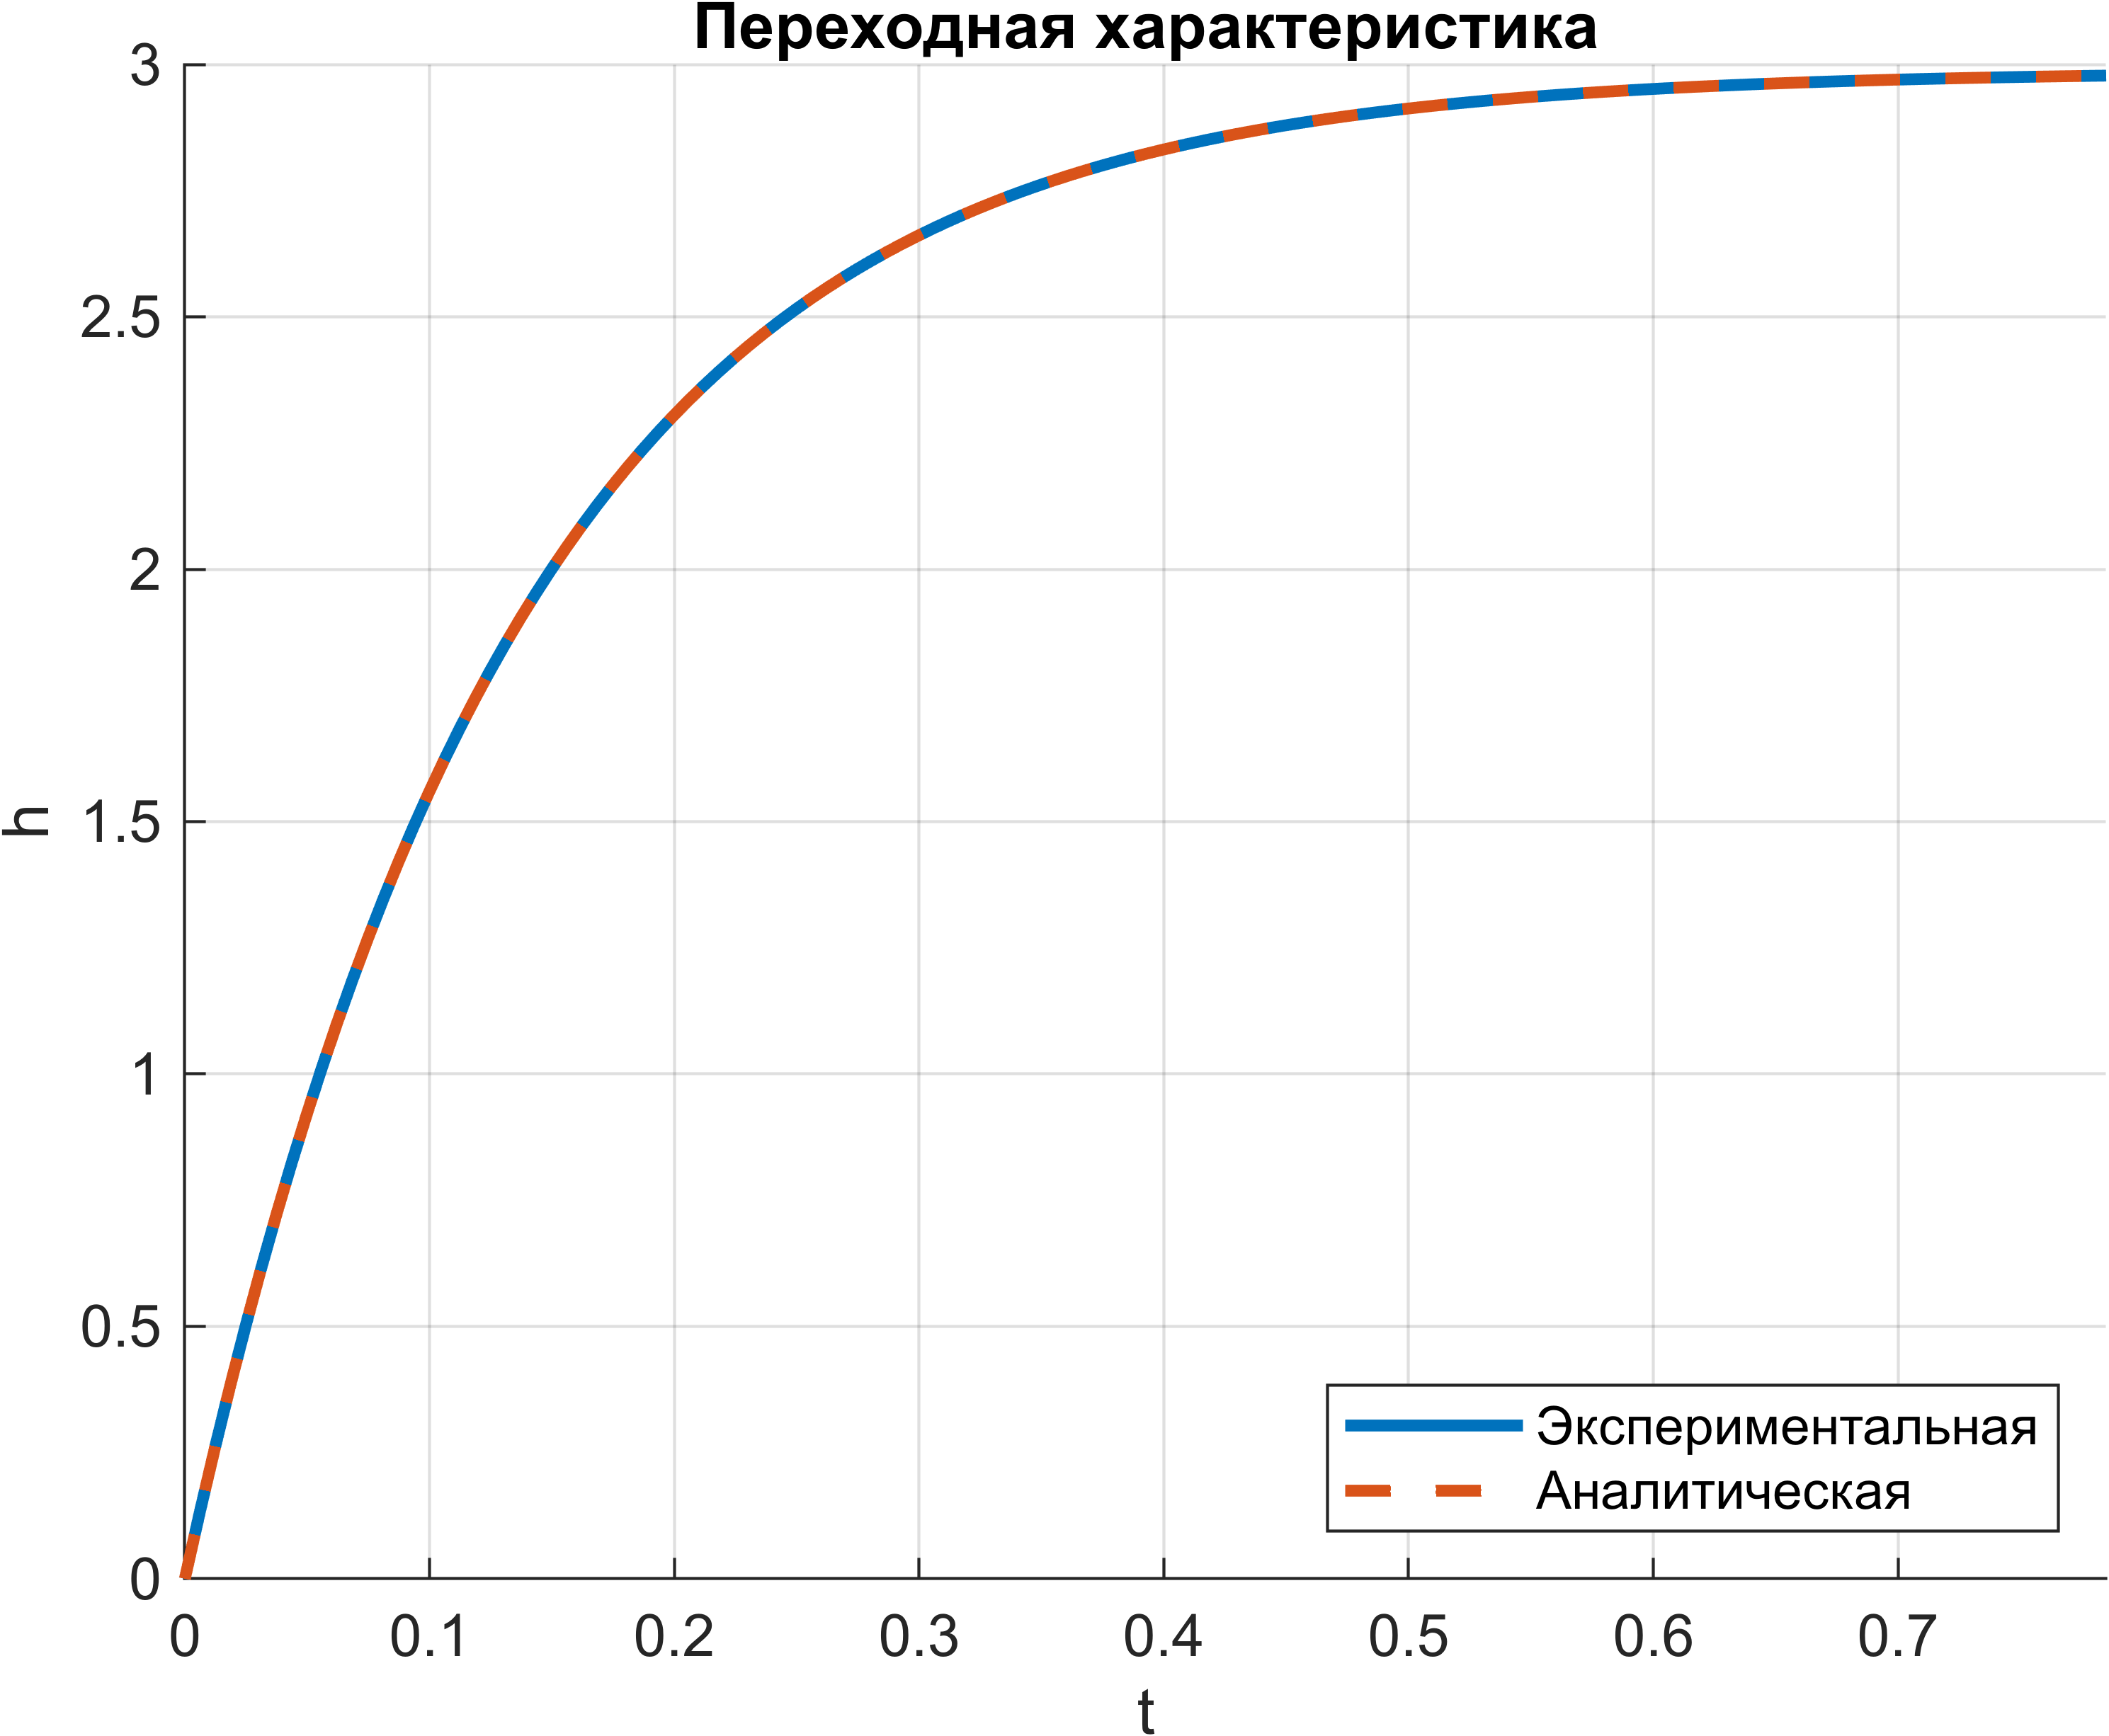
\includegraphics[width=0.75\textwidth, trim={0cm 0cm 0cm 0cm}]{../images/1_1.png}
    \caption{Переходная характеристика ДПТ}
\end{figure}

\begin{figure}[H]
    \centering
    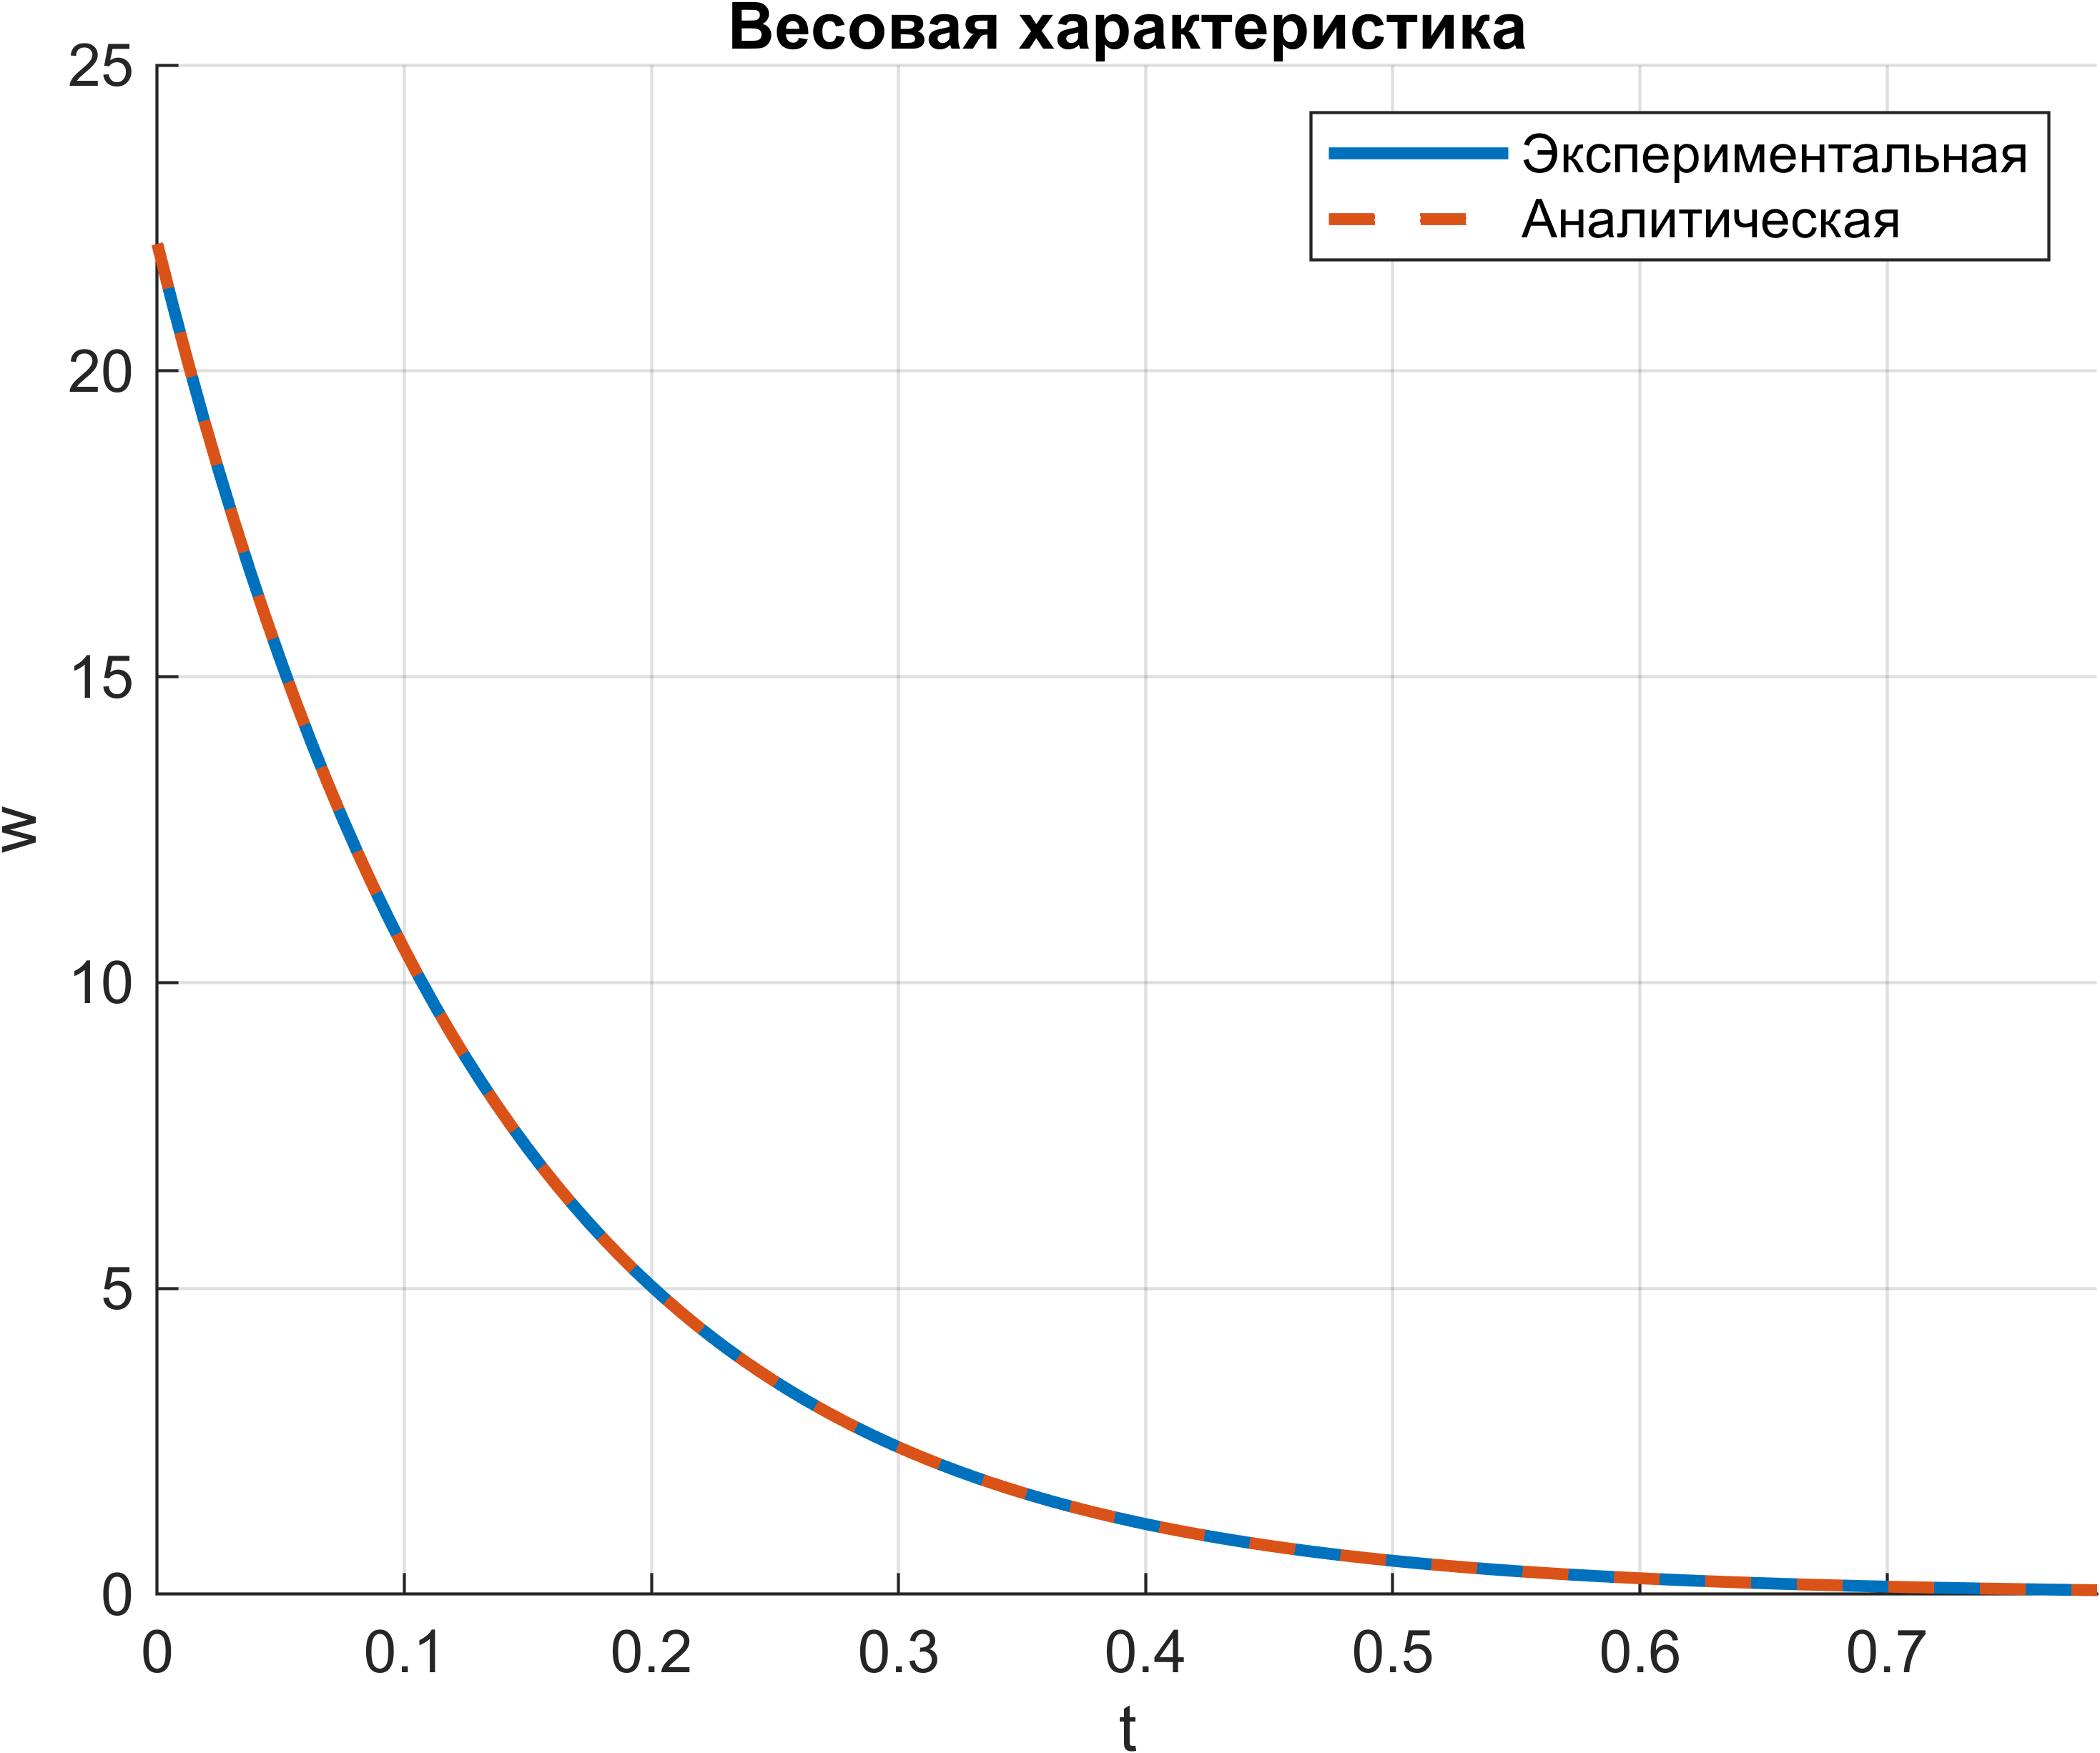
\includegraphics[width=0.75\textwidth, trim={0cm 0cm 0cm 0cm}]{../images/1_2.png}
    \caption{Весовая характеристика ДПТ}
\end{figure}

\section{Частотные характеристики}

Амплитудно-частотная характеристика - зависимость амплитуды выходного сигнала от частоты входного сигнала.
Для реального усилительного звена имеет вид:
\[
A(\omega) = \frac{K}{\sqrt{1 + \omega^2 T^2}}
\]

Логарифмическая амплитудно-частотная характеристика:
\[
L(\omega) = 20 \lg A(\omega) = 20 \lg K - 10 \lg (1 + \omega^2 T^2)
\]

Фазо-частотная характеристика - зависимость фазы выходного сигнала от частоты входного сигнала.
Для реального усилительного звена имеет вид:
\[
\phi(\omega) = -\arctan(\omega T)
\]

\begin{figure}[H]
    \centering
    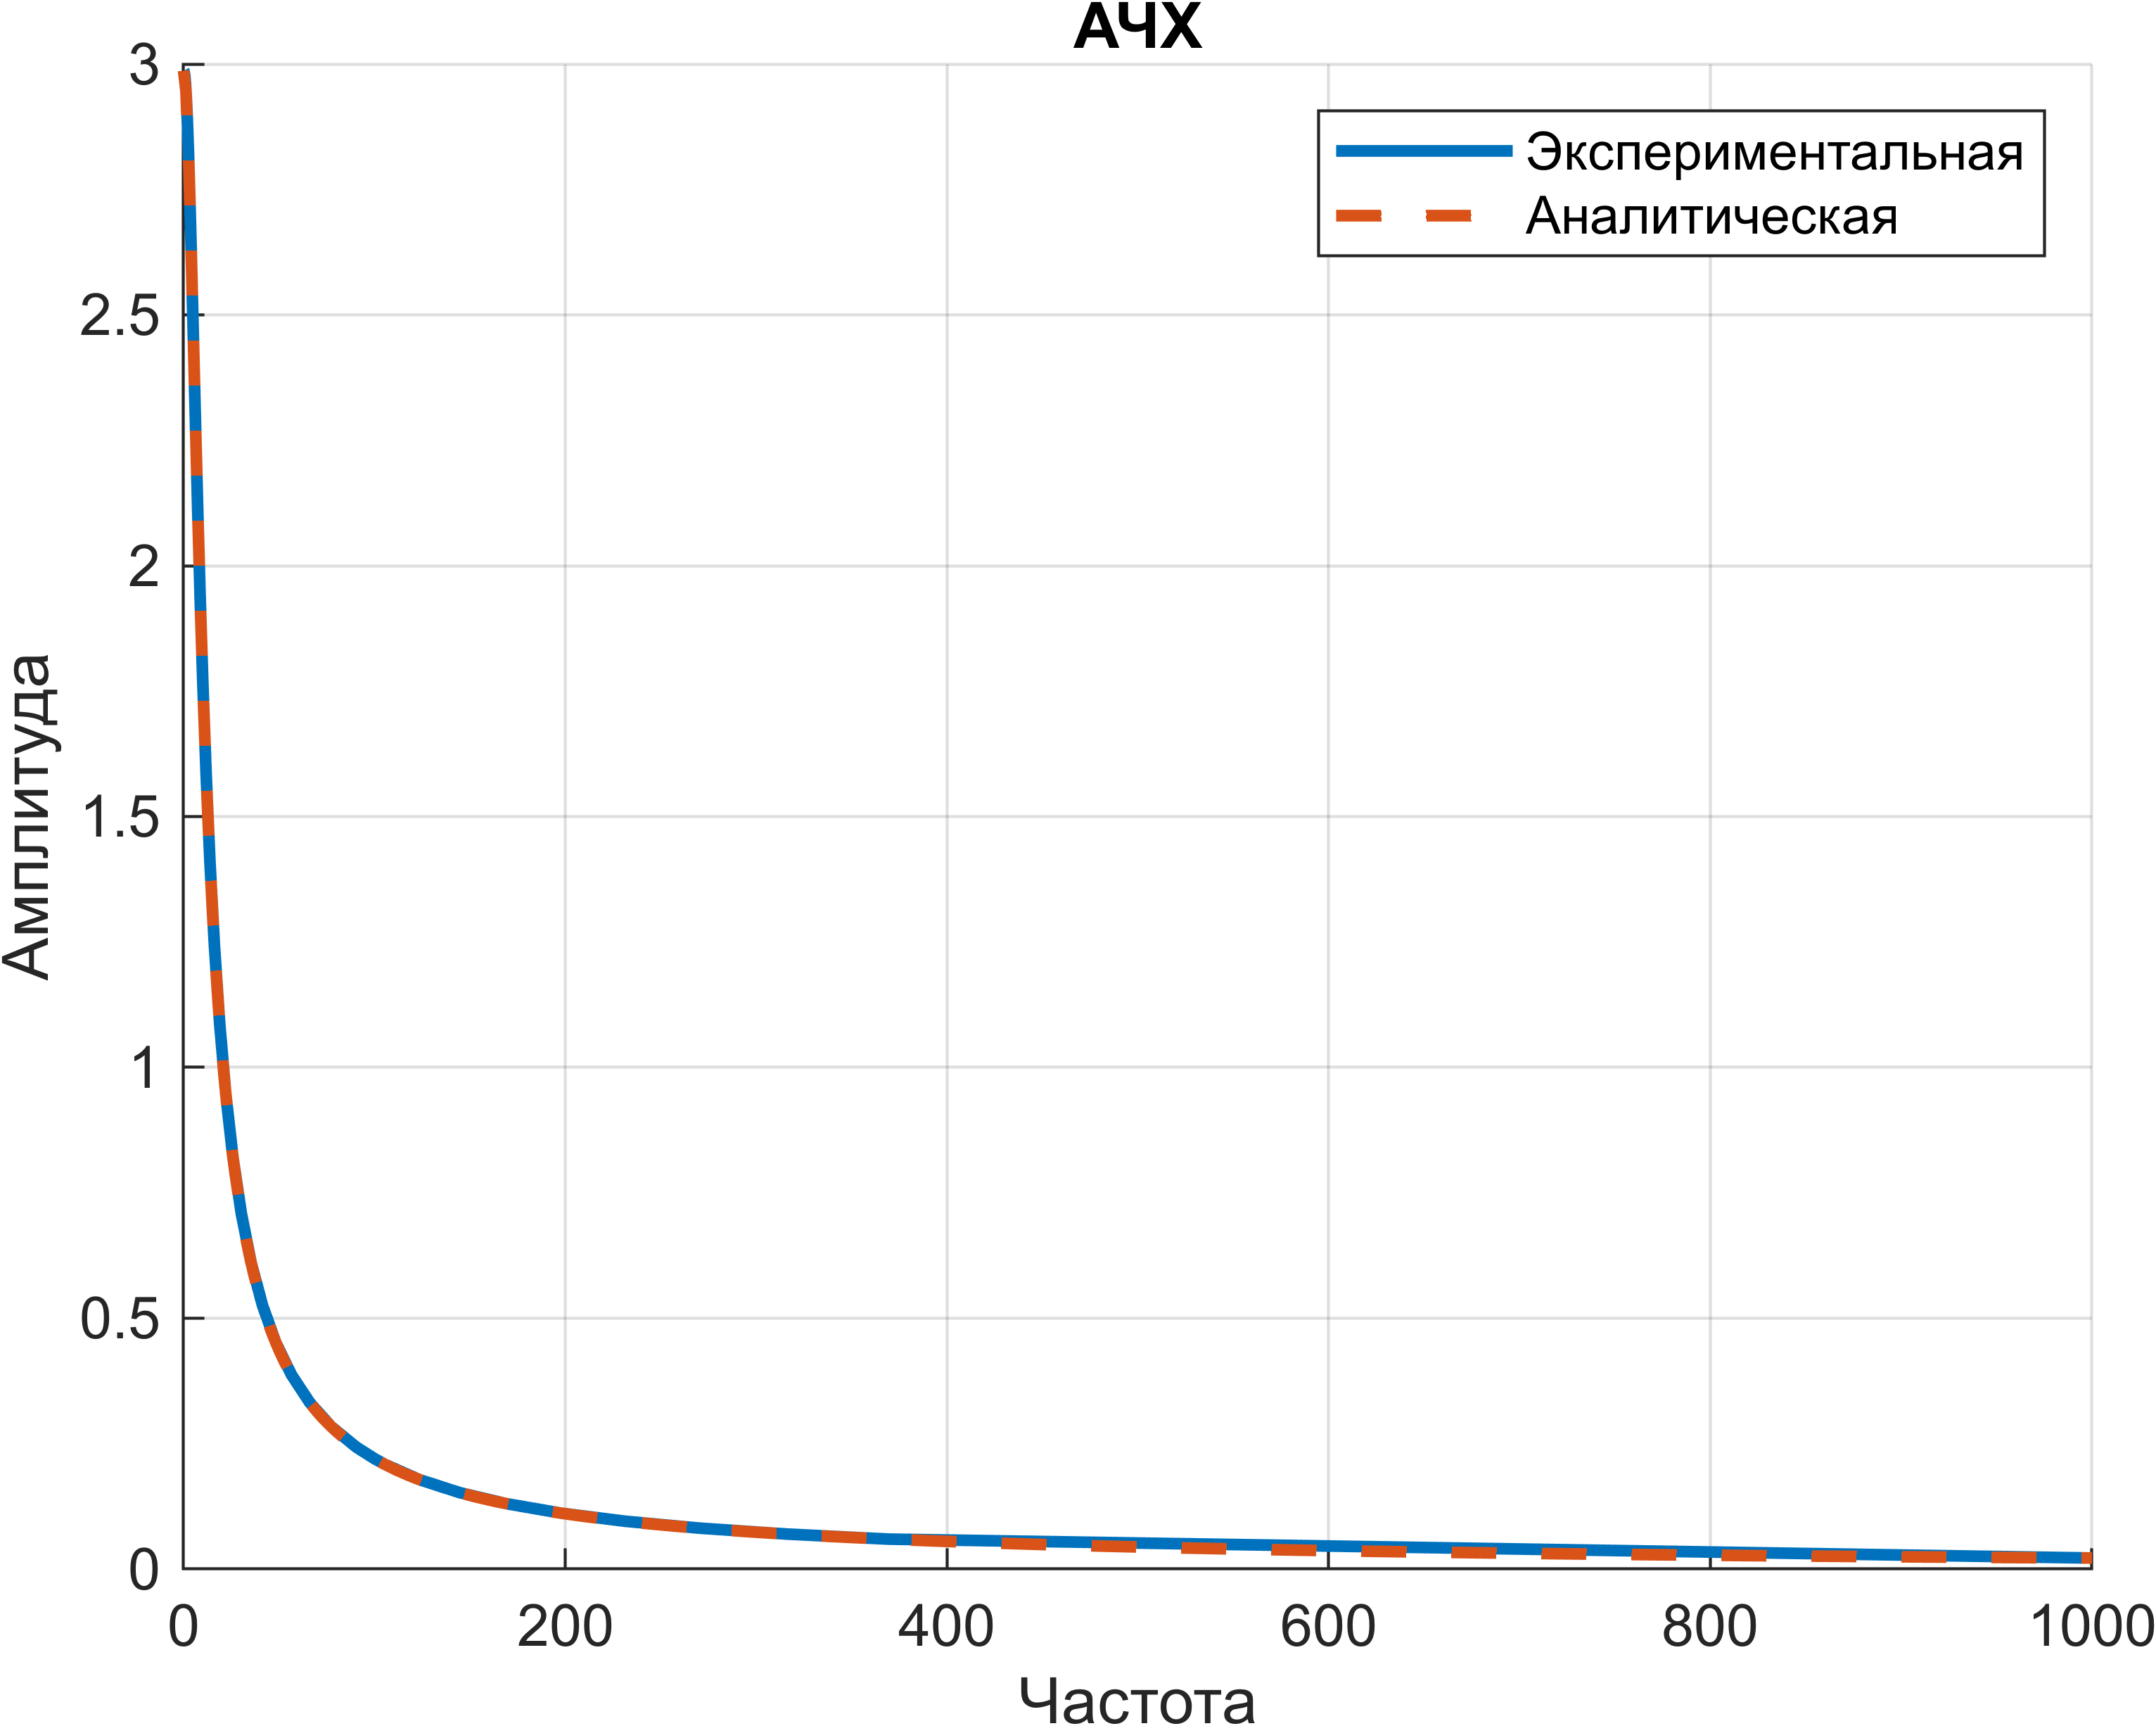
\includegraphics[width=0.75\textwidth, trim={0cm 0cm 0cm 0cm}]{../images/1_3.png}
    \caption{Амплитудно-частотная характеристика ДПТ}
\end{figure}

\begin{figure}[H]
    \centering
    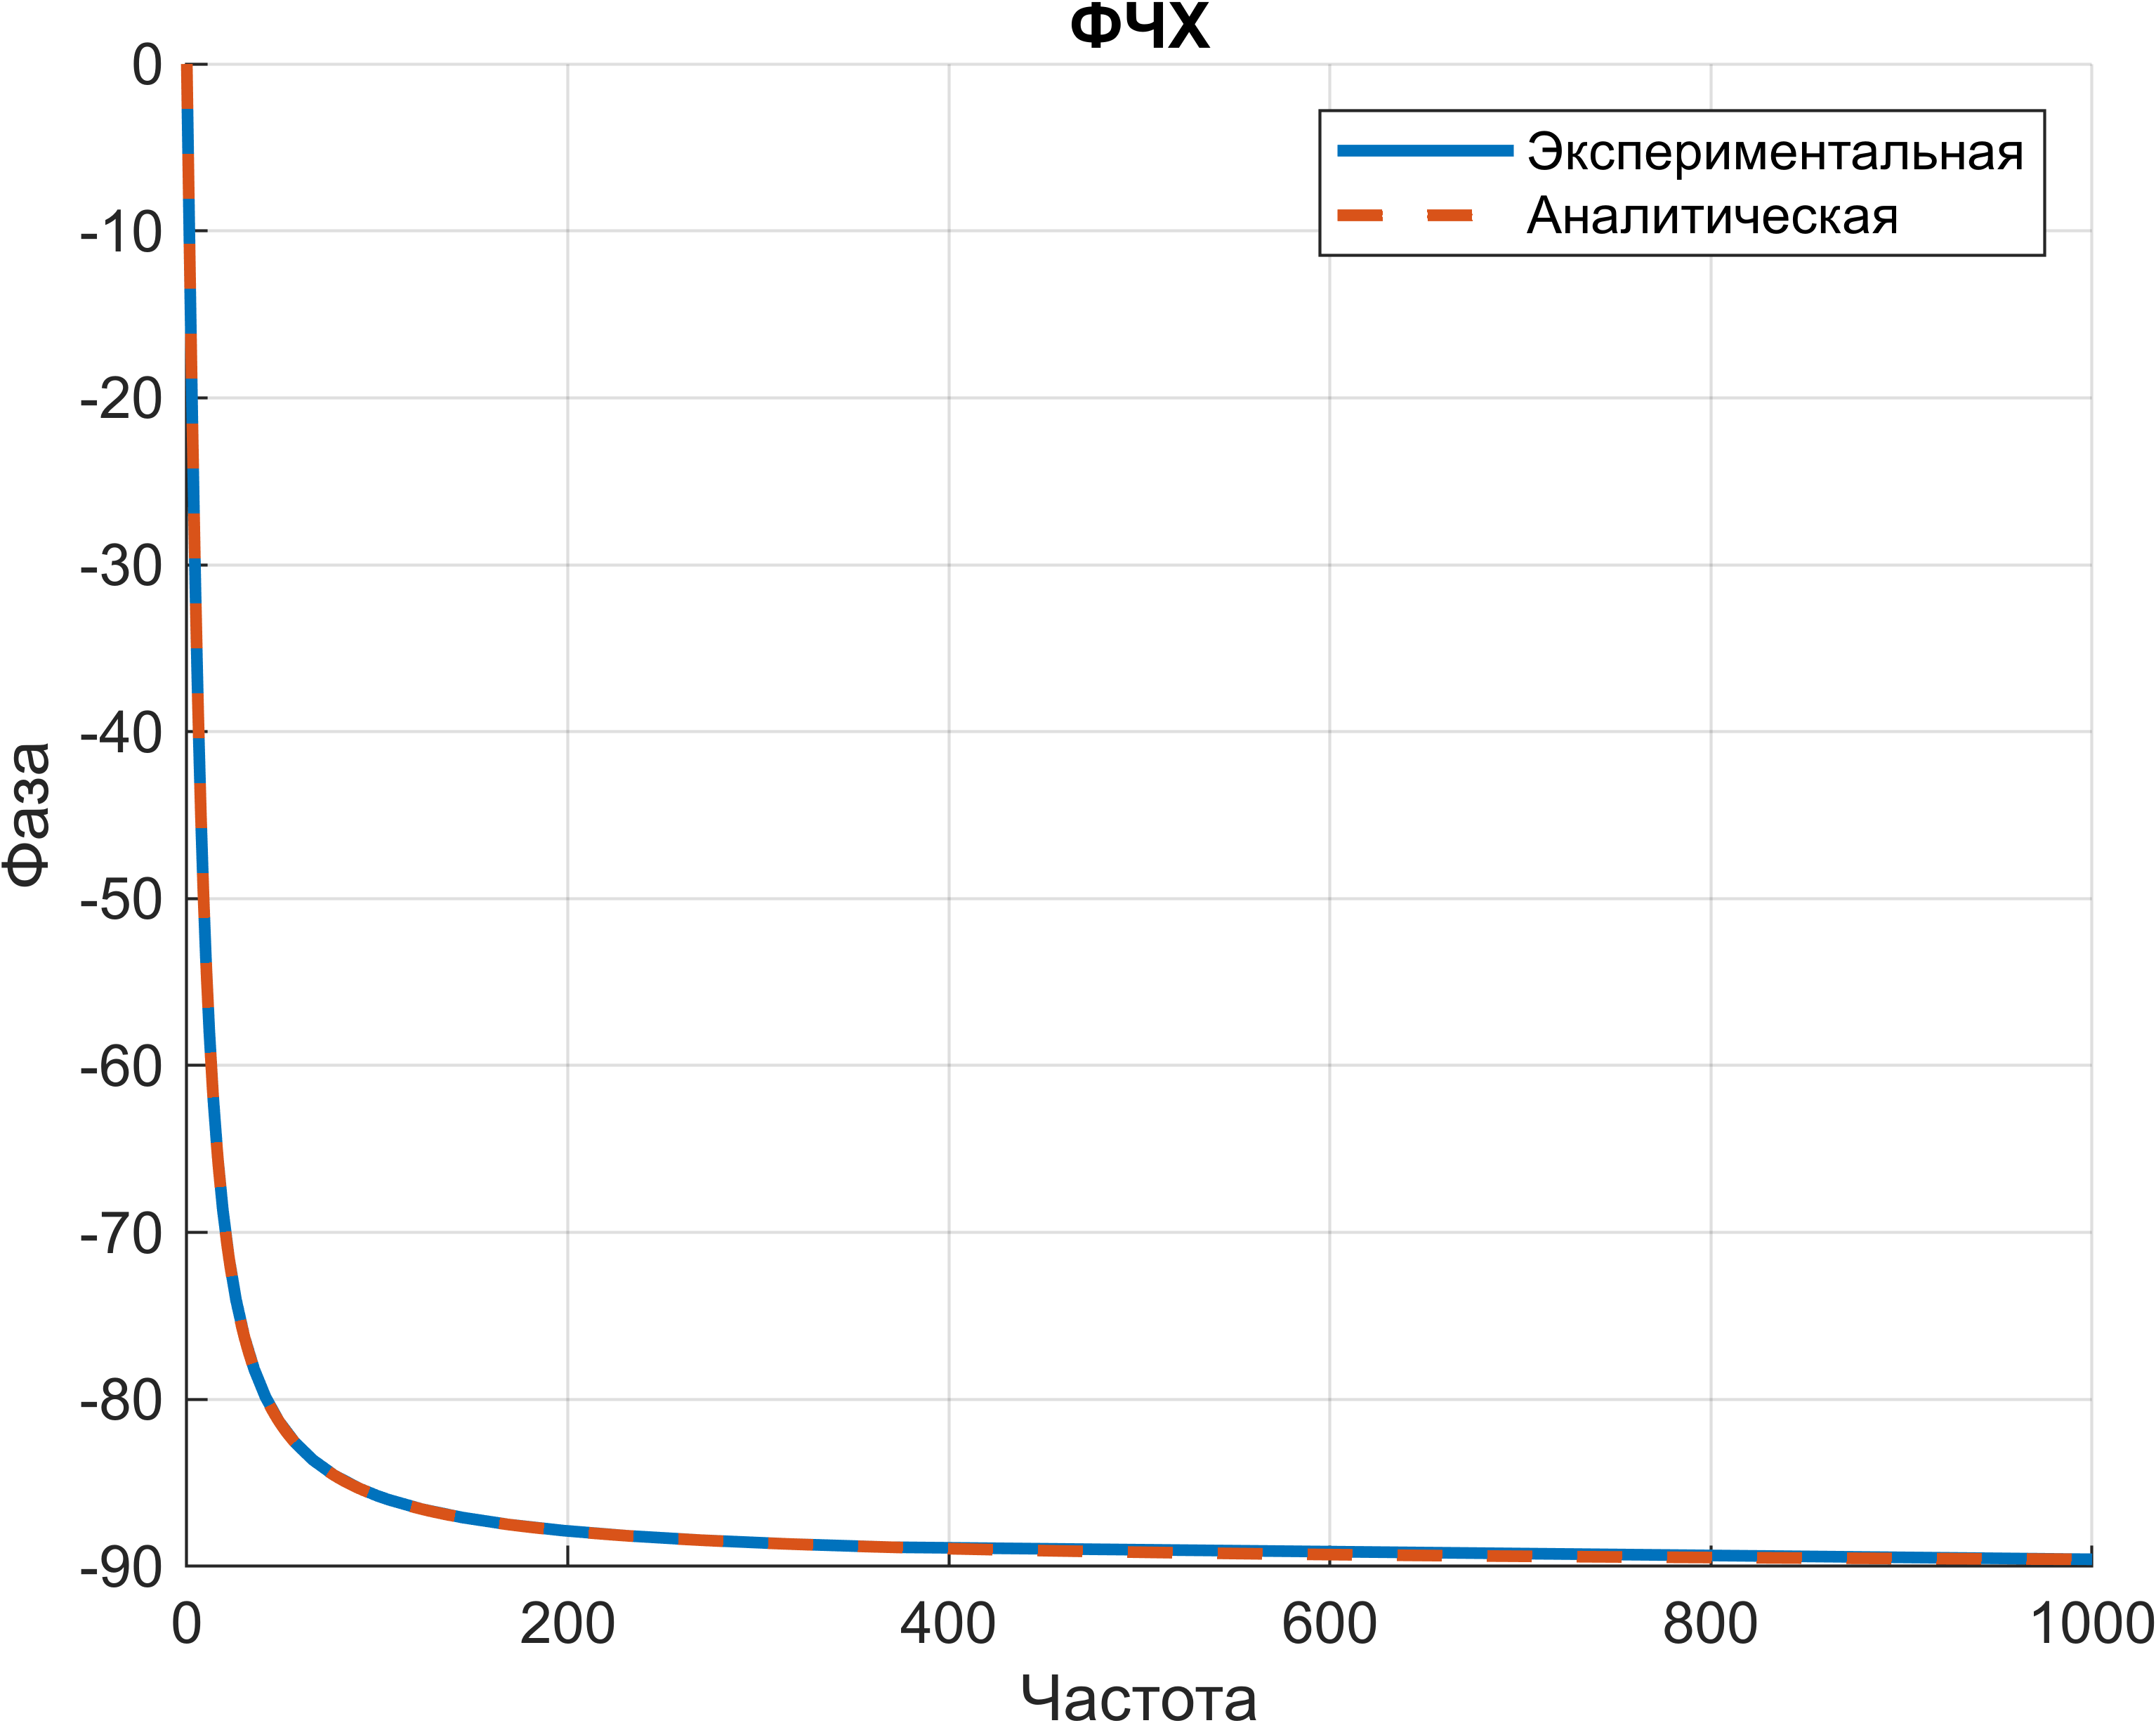
\includegraphics[width=0.75\textwidth, trim={0cm 0cm 0cm 0cm}]{../images/1_4.png}
    \caption{Фазо-частотная характеристика ДПТ}
\end{figure}

\begin{figure}[H]
    \centering
    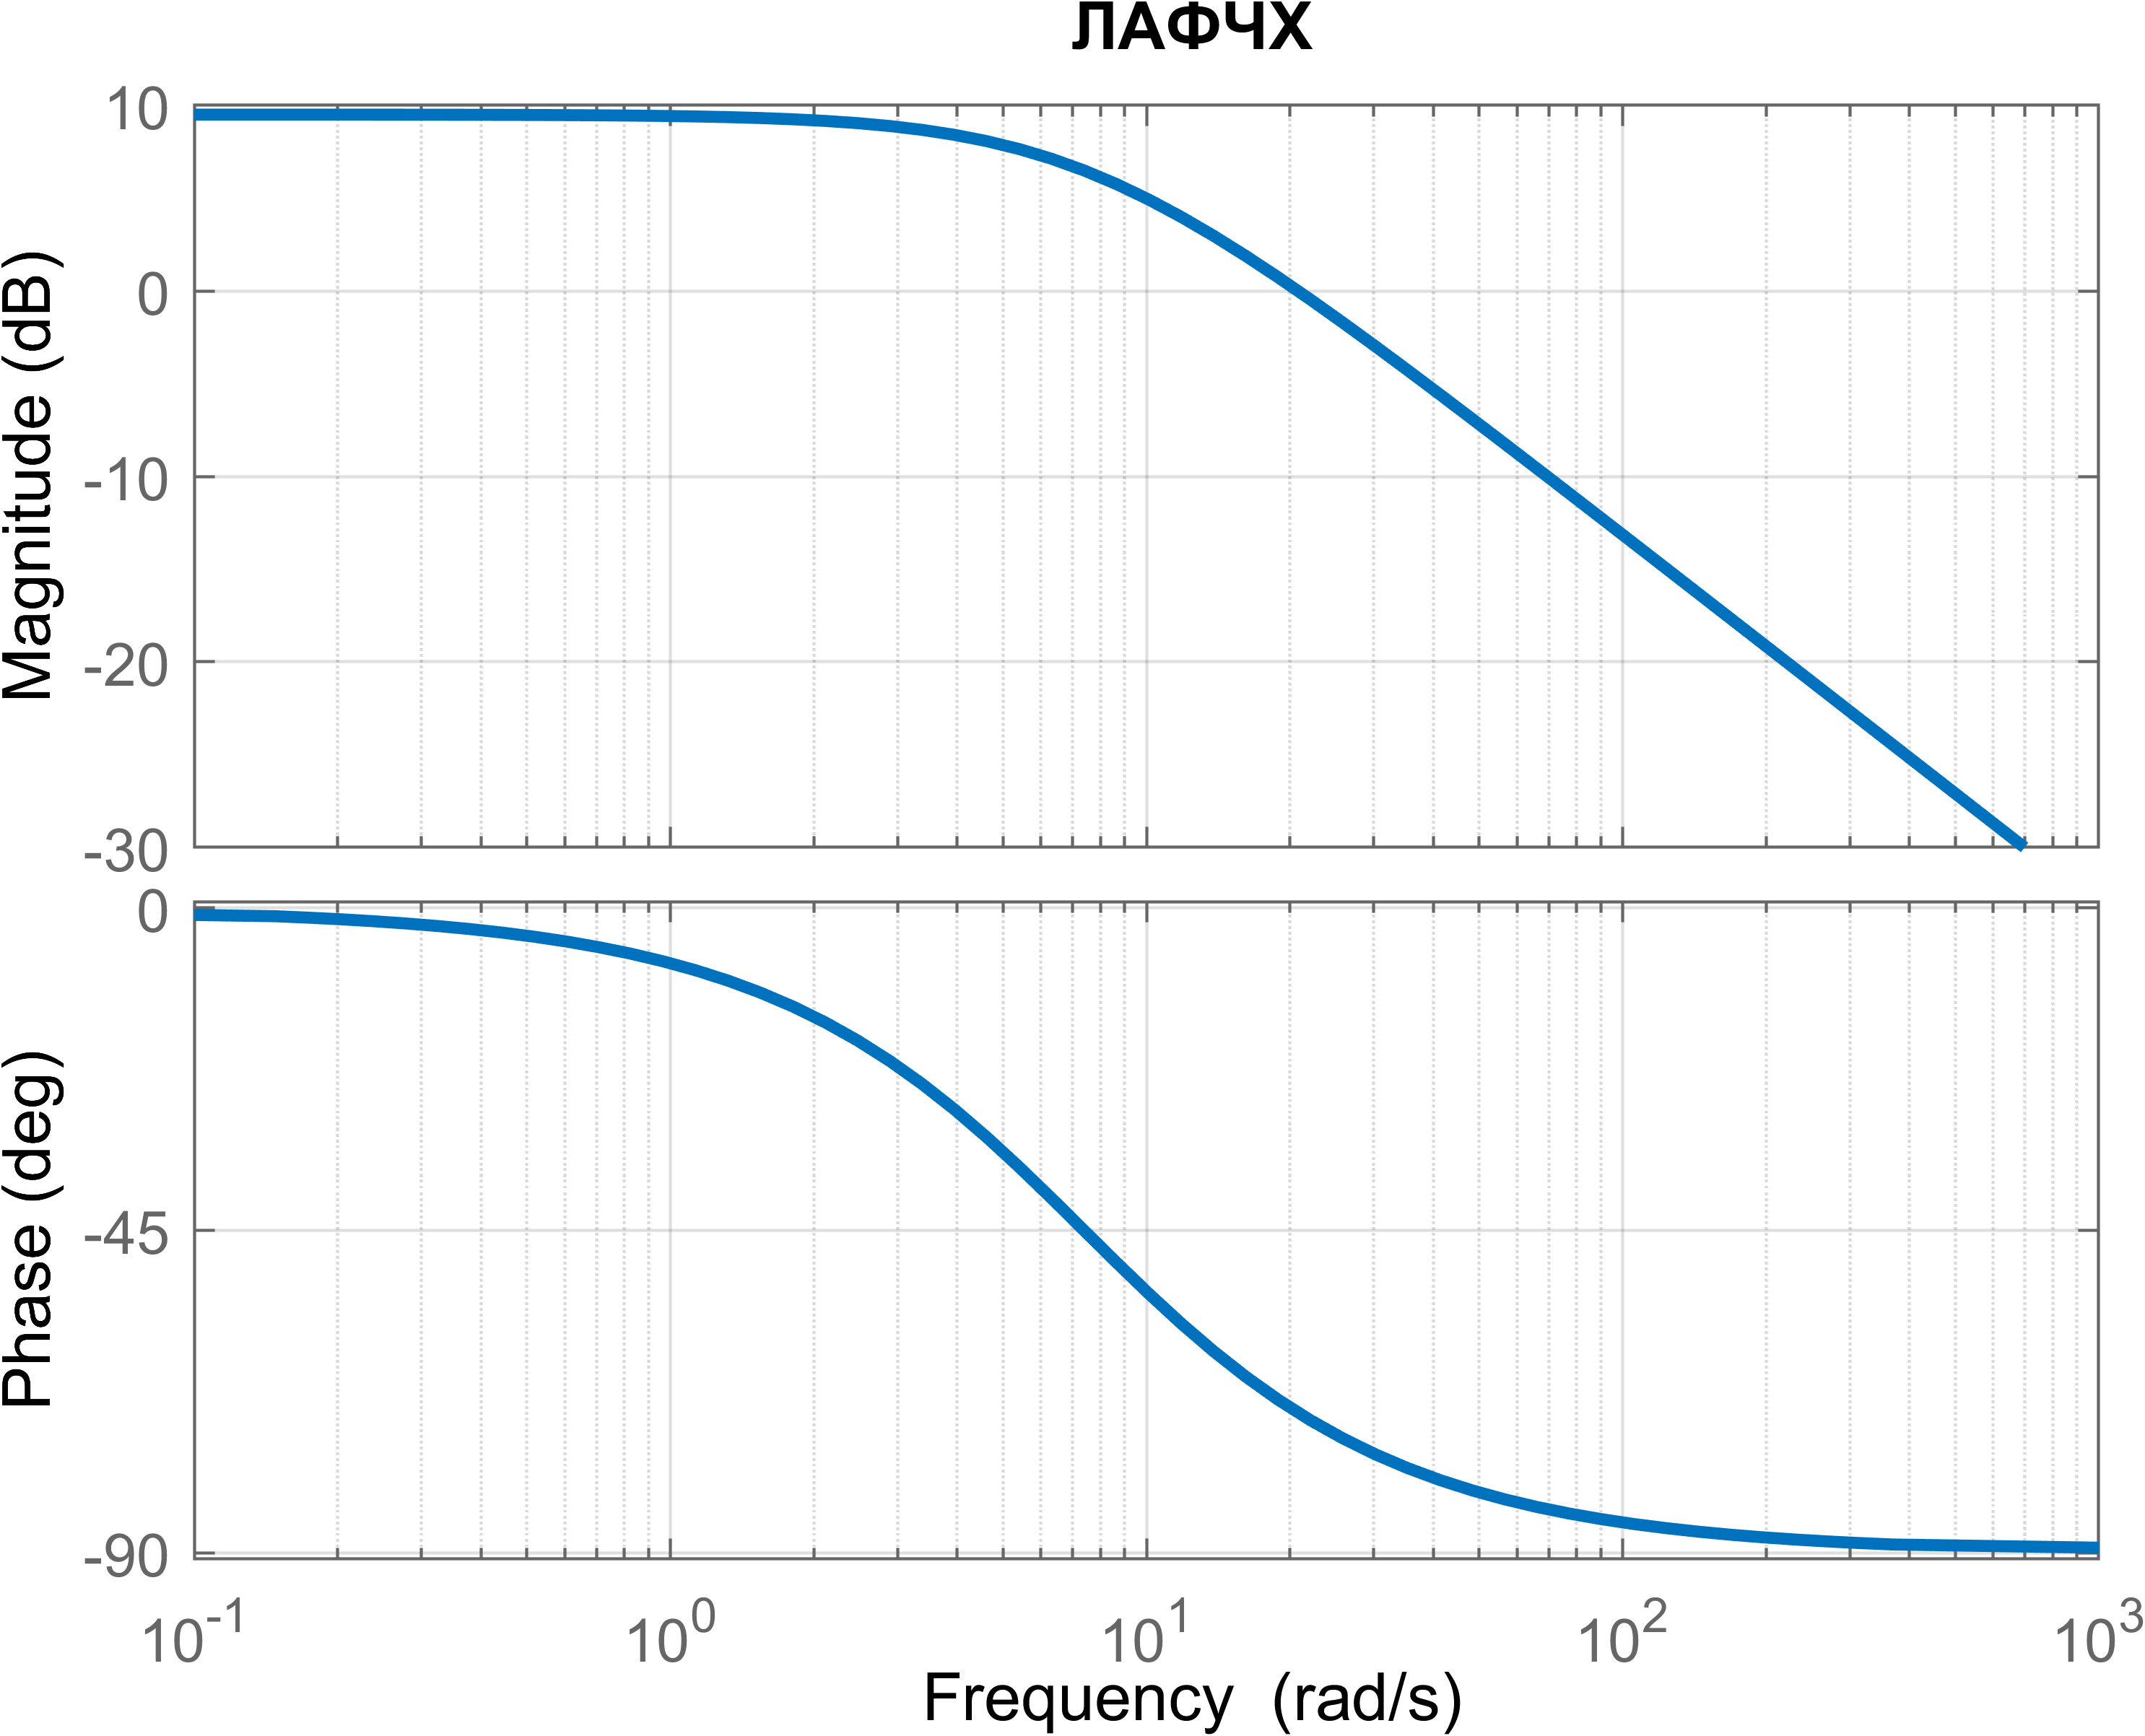
\includegraphics[width=0.75\textwidth, trim={0cm 0cm 0cm 0cm}]{../images/1_5.png}
    \caption{Логарифмическая амплитудно-фазо-частотная характеристика ДПТ}
\end{figure}

\endinput